\documentclass[11pt,a4paper]{article}
\usepackage[utf8]{inputenc}
\usepackage[T1]{fontenc}
\usepackage{amsmath,amssymb}
\usepackage{geometry}
\geometry{margin=2.5cm}
\usepackage{graphicx}
\usepackage{hyperref}
\usepackage{listings}
\usepackage{xcolor}
\usepackage{tikz}
\usetikzlibrary{automata,positioning,arrows.meta,shapes.multipart}

% Code listing style
\lstset{
  language=Python,
  basicstyle=\ttfamily\small,
  keywordstyle=\color{blue}\bfseries,
  commentstyle=\color{gray}\itshape,
  stringstyle=\color{orange},
  frame=single,
  breaklines=true,
  numbers=left,
  numberstyle=\tiny\color{gray}
}

\title{Multiplayer Entity Model \& State Transition Documentation\\
\large Core Systems -- RTS Engine (Godot 4.x / GDScript)}
\author{Core Systems Engineering Team}
\date{March 2026}

\begin{document}
\maketitle
\tableofcontents
\newpage

% =====================================================================
\section{Multiplayer Entity Model}
% =====================================================================

\subsection{Overview}

The Multiplayer Entity Model introduces a \texttt{player\_id} attribute across
all game entities, enabling ownership-based command validation, friendly/hostile
discrimination in combat, and per-player sense queries. Every unit, building,
and resource in the game world is assigned to a player (or marked neutral).

\subsection{Entity Hierarchy}

The inheritance hierarchy ensures all game objects share the IDamageable
contract:

\begin{center}
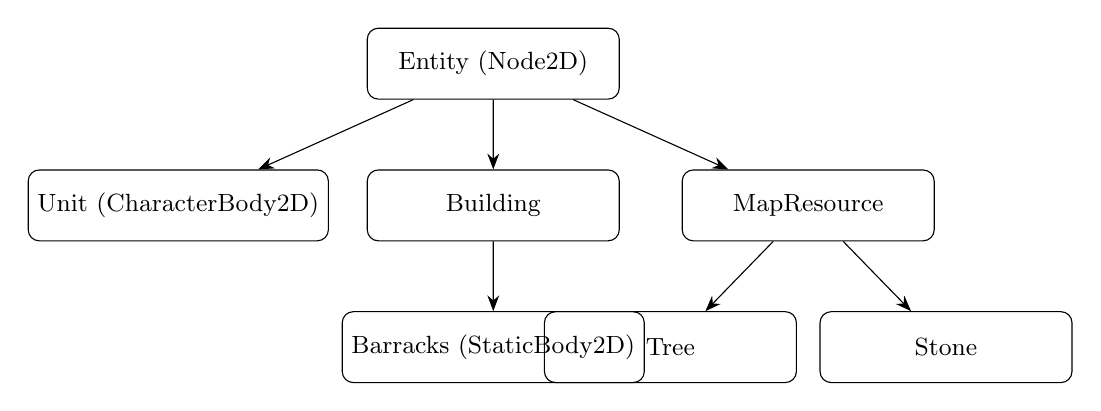
\begin{tikzpicture}[
    every node/.style={draw, rounded corners, minimum width=3.2cm, minimum height=0.9cm, font=\small},
    level 1/.style={sibling distance=4cm},
    level 2/.style={sibling distance=3.5cm},
    edge from parent/.style={draw,-{Stealth[length=2mm]}},
    level distance=1.8cm
]
\node {Entity (Node2D)}
    child {node {Unit (CharacterBody2D)}
    }
    child {node {Building}
        child {node {Barracks (StaticBody2D)}}
    }
    child {node {MapResource}
        child {node {Tree}}
        child {node {Stone}}
    };
\end{tikzpicture}
\end{center}

\subsection{Player Ownership Attributes}

\begin{center}
\begin{tabular}{|l|l|l|p{6cm}|}
\hline
\textbf{Class} & \textbf{Attribute} & \textbf{Type} & \textbf{Description} \\
\hline
Entity          & \texttt{player\_id}  & \texttt{int} & Owner player. $-1$ = neutral/environment. \\
Entity          & \texttt{entity\_id}  & \texttt{int} & Unique identifier for AI lookups. \\
Entity          & \texttt{max\_health} & \texttt{int} & Maximum hit points. \\
Unit            & \texttt{attack\_range}   & \texttt{float} & Proximity scan radius for combat. \\
Unit            & \texttt{attack\_damage}  & \texttt{int}   & Damage applied per attack tick. \\
Unit            & \texttt{attack\_cooldown}& \texttt{float} & Seconds between attacks. \\
Barracks        & \texttt{player\_id}  & \texttt{int} & Owner of the barracks. \\
MapResource     & \texttt{player\_id}  & \texttt{int} & Always $-1$ (neutral). \\
\hline
\end{tabular}
\end{center}

\subsection{IDamageable Interface}

The \texttt{IDamageable} interface defines the universal damage contract.
Any object that can receive damage implements:

\begin{center}
\begin{tabular}{|l|l|p{7cm}|}
\hline
\textbf{Method} & \textbf{Return} & \textbf{Description} \\
\hline
\texttt{take\_damage(amount)} & \texttt{void} & Reduce HP by \texttt{amount}. Triggers \texttt{die()} if $\leq 0$. \\
\texttt{get\_current\_health()} & \texttt{int} & Current hit points. \\
\texttt{is\_alive()} & \texttt{bool} & True if HP $> 0$. \\
\texttt{get\_player\_id()} & \texttt{int} & Owner's player ID. \\
\hline
\end{tabular}
\end{center}

Compliance is verified at runtime via duck-typing:

\begin{lstlisting}[language=Python,caption={IDamageable.is\_implemented\_by()}]
static func is_implemented_by(obj: Variant) -> bool:
    if obj == null:
        return false
    return (
        obj.has_method("get_current_health")
        and obj.has_method("is_alive")
        and obj.has_method("take_damage")
        and obj.has_method("get_player_id")
    )
\end{lstlisting}

\subsection{Ownership Validation in ActionGateway}

Before any command is executed, the ActionGateway validates:

$$
\texttt{unit.player\_id} \stackrel{?}{=} \texttt{request.player\_id}
$$

If the check fails, the request is rejected and a \texttt{[OWNERSHIP\_ERR]}
log entry is emitted. When \texttt{requesting\_player\_id} is $-1$, the check
is skipped for backwards compatibility.

% =====================================================================
\section{State Transition Diagrams}
% =====================================================================

\subsection{Unit Command Lifecycle}

\begin{center}
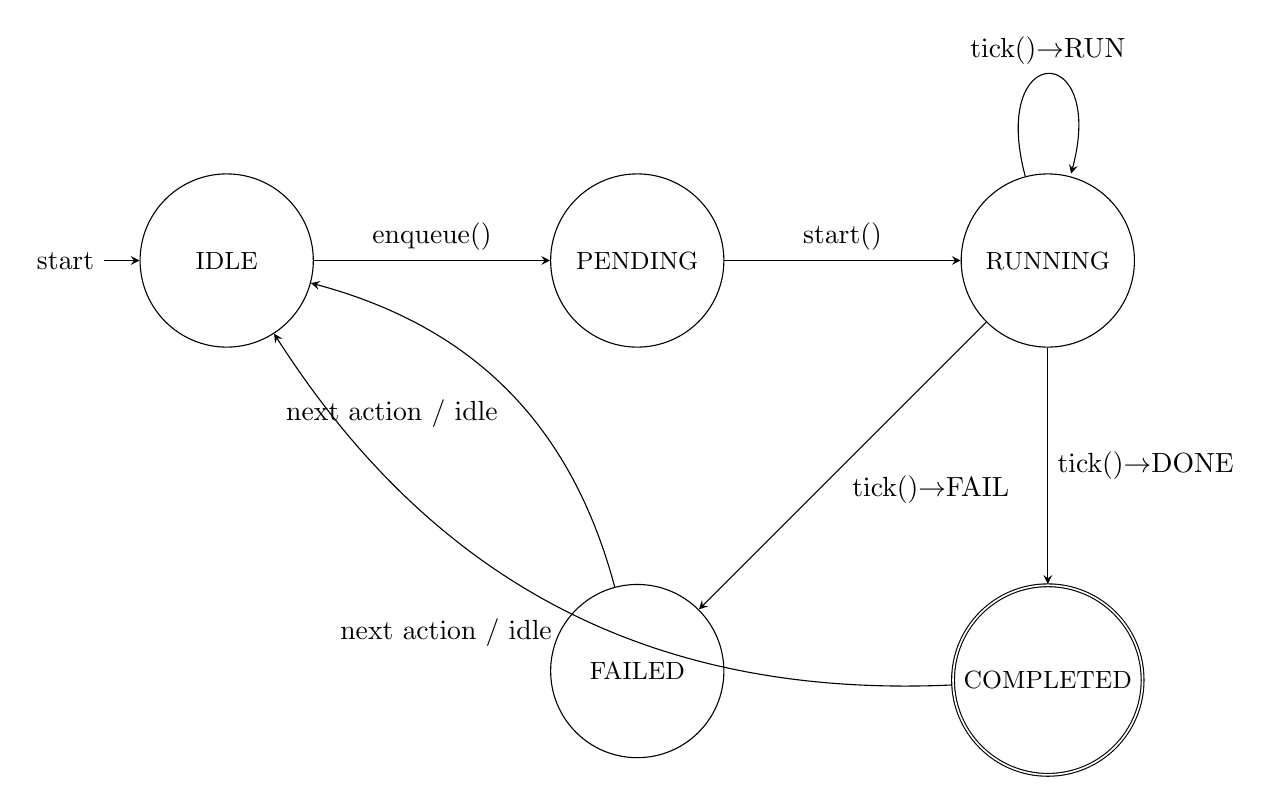
\begin{tikzpicture}[
    ->,>=stealth,
    node distance=3cm,
    every state/.style={draw, rounded corners, minimum width=2.2cm, minimum height=0.8cm, font=\small},
    auto
]
    \node[state, initial]   (idle)     {IDLE};
    \node[state]            (pending)  [right=of idle]     {PENDING};
    \node[state]            (running)  [right=of pending]  {RUNNING};
    \node[state, accepting] (done)     [below=of running]  {COMPLETED};
    \node[state]            (failed)   [below=of pending]  {FAILED};

    \path (idle)    edge node {enqueue()} (pending)
          (pending) edge node {start()}   (running)
          (running) edge node {tick()$\rightarrow$DONE} (done)
          (running) edge node {tick()$\rightarrow$FAIL} (failed)
          (running) edge [loop above] node {tick()$\rightarrow$RUN} (running)
          (done)    edge [bend left] node {next action / idle} (idle)
          (failed)  edge [bend right] node {next action / idle} (idle);
\end{tikzpicture}
\end{center}

\subsection{Chop-and-Return Composite State Machine}

The \texttt{go\_chop\_tree\_and\_return()} command is a multi-step autonomous
sequence managed internally by the ActionGateway:

\begin{center}
\begin{tikzpicture}[
    ->,>=stealth,
    node distance=2.8cm,
    every state/.style={draw, rounded corners, minimum width=2.8cm, minimum height=0.8cm, font=\small},
    auto
]
    \node[state, initial]   (start)    {API Call};
    \node[state]            (move1)    [right=of start]    {MOVE to Tree};
    \node[state]            (harvest)  [right=of move1]    {HARVEST};
    \node[state]            (move2)    [below=of harvest]  {RETURN to Base};
    \node[state, accepting] (idle)     [below=of move1]    {IDLE};

    \path (start)   edge node {\footnotesize enqueue} (move1)
          (move1)   edge node {\footnotesize arrived} (harvest)
          (harvest) edge node {\footnotesize queue\_empty} (move2)
          (move2)   edge node {\footnotesize queue\_empty} (idle);
\end{tikzpicture}
\end{center}

Key design: the \texttt{queue\_empty} signal triggers the next phase
\emph{internally}, so the AI team only sends one initial request.

\subsection{Combat State Machine}

\begin{center}
\begin{tikzpicture}[
    ->,>=stealth,
    node distance=3cm,
    every state/.style={draw, rounded corners, minimum width=2.5cm, minimum height=0.8cm, font=\small},
    auto
]
    \node[state, initial]   (scan)    {SCAN};
    \node[state]            (chase)   [right=of scan]    {CHASE};
    \node[state]            (attack)  [right=of chase]   {ATTACK};
    \node[state, accepting] (done)    [below=of chase]   {COMPLETED};

    \path (scan)   edge node {\footnotesize hostile found} (chase)
          (scan)   edge [bend right=40] node[below] {\footnotesize no hostiles} (done)
          (chase)  edge node {\footnotesize in range} (attack)
          (chase)  edge [loop above] node {\footnotesize moving} (chase)
          (attack) edge [loop above] node {\footnotesize cooldown tick} (attack)
          (attack) edge node[right] {\footnotesize target dead} (scan)
          (attack) edge [bend left=20] node {\footnotesize no hostiles} (done);
\end{tikzpicture}
\end{center}

% =====================================================================
\section{API Reference Updates}
% =====================================================================

\subsection{ActionGateway -- New Commands}

\begin{center}
\begin{tabular}{|l|p{8cm}|}
\hline
\textbf{Method} & \textbf{Description} \\
\hline
\texttt{go\_chop\_tree\_and\_return(uid, tid, pid)} & Composite: move $\rightarrow$ harvest $\rightarrow$ return to barracks $\rightarrow$ idle. \\
\texttt{attack\_target(uid, tid, pid)} & Move to and attack a specific hostile entity. \\
\texttt{attack\_move(uid, dest, pid)} & Move to position, auto-attack hostiles in range. \\
\texttt{get\_idle\_units(pid)} & Pass-through to SenseAPI. \\
\texttt{get\_busy\_units(pid)} & Pass-through to SenseAPI. \\
\hline
\end{tabular}
\end{center}

All commands accept \texttt{requesting\_player\_id} as the last parameter.
Set to $-1$ to skip ownership validation (test/single-player mode).

\subsection{SenseAPI -- New Queries}

\begin{center}
\begin{tabular}{|l|l|p{6cm}|}
\hline
\textbf{Method} & \textbf{Return} & \textbf{Description} \\
\hline
\texttt{get\_idle\_units(pid)} & \texttt{Array[int]} & Entity IDs of all idle units for player \texttt{pid}. \\
\texttt{get\_busy\_units(pid)} & \texttt{Array[int]} & Entity IDs of all busy units for player \texttt{pid}. \\
\hline
\end{tabular}
\end{center}

\subsection{Logging Tags}

\begin{center}
\begin{tabular}{|l|p{8cm}|}
\hline
\textbf{Tag} & \textbf{Usage} \\
\hline
\texttt{[OWNERSHIP\_ERR]} & Cross-player command rejected. \\
\texttt{[COMBAT\_LOG]}    & Damage dealt/received, unit destroyed, combat state changes. \\
\texttt{[IDLE\_REPORT]}   & Unit idle/busy transitions, chop-and-return completion. \\
\hline
\end{tabular}
\end{center}

% =====================================================================
\section{Sandbox Verification Matrix}
% =====================================================================

\begin{center}
\begin{tabular}{|c|p{5cm}|p{5cm}|c|}
\hline
\textbf{Test} & \textbf{Scenario} & \textbf{Expected Outcome} & \textbf{Tag} \\
\hline
1 & Player 1 commands Player 0's unit & Rejected with \texttt{[OWNERSHIP\_ERR]} & PASS/FAIL \\
2 & Player 0 commands own unit & Accepted, unit moves & PASS/FAIL \\
3 & \texttt{get\_busy\_units(0)} during action & Returns non-empty array & PASS/FAIL \\
4 & \texttt{go\_chop\_tree\_and\_return()} & Unit returns to barracks, \texttt{is\_idle = true} & PASS/FAIL \\
5 & Unit distance to barracks after return & $< 50.0$ units & PASS/FAIL \\
\hline
\end{tabular}
\end{center}

\end{document}
